\documentclass[xcolor=dvipsnames]{beamer}
\mode<presentation> {
	\usetheme{Madrid}
}
% 
\setbeamercolor{normal text}{fg=black,bg=white}

\setbeamercolor{title}{fg=white}

\setbeamercolor{frametitle}{
	bg=black!90,
	fg=white
}

\setbeamercolor{structure}{
	fg=teal!70!black
}

\setbeamertemplate{blocks}[rounded][shadow=true]

% ===== DEFINICJA =====

\newenvironment{definicja}[1][]
{
	\setbeamercolor{block title}{
		bg=teal!70!black,
		fg=white
	}
	\setbeamercolor{block body}{
		bg=teal!5,
		fg=black
	}
	\begin{block}{Definicja #1}
	}
	{
	\end{block}
}

% ===== TWIERDZENIE =====

\newenvironment{twierdzenie}[1][]
{
	\setbeamercolor{block title}{
		bg=teal!70!black,
		fg=white
	}
	\setbeamercolor{block body}{
		bg=teal!5,
		fg=black
	}
	\begin{block}{Twierdzenie #1}
	}
	{
	\end{block}
}

% ===== UWAGA =====

\newenvironment{uwaga}[1][]
{
	\setbeamercolor{block title}{
		bg=orange!85!black,
		fg=white
	}
	\setbeamercolor{block body}{
		bg=orange!8,
		fg=black
	}
	\begin{block}{Uwaga #1}
	}
	{
	\end{block}
}

% ===== PRZYKLAD =====

\newenvironment{przyklad}[1][]
{
	\setbeamercolor{block title}{
		bg=green!50!black,
		fg=white
	}
	\setbeamercolor{block body}{
		bg=green!5,
		fg=black
	}
	\begin{block}{Przykład #1}
	}
	{
	\end{block}
}

% ===== WNIOSEK =====

\newenvironment{wniosek}[1][]
{
	\setbeamercolor{block title}{
		bg=violet!70!black,
		fg=white
	}
	\setbeamercolor{block body}{
		bg=violet!5,
		fg=black
	}
	\begin{block}{Wniosek #1}
	}
	{
	\end{block}
}

% ===== PROBLEM =====

\newenvironment{problemo}[1][]
{
	\setbeamercolor{block title}{
		bg=red!70!black,
		fg=white
	}
	\setbeamercolor{block body}{
		bg=red!5,
		fg=black
	}
	\begin{block}{Problem #1}
	}
	{
	\end{block}
}

\usepackage[polish]{babel}
\usepackage[MeX]{polski}
\usepackage[utf8]{inputenc}
\usepackage{calligra}
\usepackage[T1]{fontenc}
\usecolortheme{default}
% \setbeamertemplate{caption}{\raggedright\insertcaption\par}
\usepackage{graphicx}
\usepackage{tikz}
\usetikzlibrary{calc}
\bibliographystyle{plain}
\usepackage{qrcode}

\title[Matematyka Czcionek]{Matematyka czcionek - wprowadzenie do krzywych Béziera}
\date{}
\author[]{Adrian Madajewski}

\titlegraphic{
	\vspace{-4.0em}
	
\includegraphics[width=0.45\textwidth]{uam_logo_bezier.jpg}
}

\begin{document}
	
	\begin{frame}
		\titlepage
	\end{frame}
	
	\begin{frame}{Cel prezentacji}
		\centering
		{\usefont{T1}{lmss}{b}{n}\scalebox{10}{B}}
	\end{frame}
	
	\begin{frame}{Grafika rastrowa, a wektorowa}
		\begin{itemize}
			\item \textbf{Grafika rastrowa:}
			\begin{itemize}
				\item Obraz jako siatka pikseli: $\{(x,y) \rightarrow kolor\}$
				\item Zależna od rozdzielczości
				\item Skalowanie $\Rightarrow$ utrata jakości
			\end{itemize}
			
			\vspace{0.5em}
			
			\pause
			
			\item \textbf{Grafika wektorowa:}
			\begin{itemize}
				\item Obraz jako zbiór krzywych i figur geometrycznych
				\item Niezależna od rozdzielczości
				\item Skalowanie $\Rightarrow$ brak utraty jakości
			\end{itemize}
		\end{itemize}
		
		\pause
		
		\begin{wniosek}
			Grafika wektorowa wymaga od nas podania \emph{przepisu} jak rysować kształty.
		\end{wniosek}
		
	\end{frame}
	
	\begin{frame}{Krzywa parametryczna}
		
		\begin{definicja}
			\textbf{Krzywa parametryczna} w $\mathbb{R}^2$ to funkcja $F : [a,b] \to \mathbb{R}^2$
			\[
			F(t) = (x(t), y(t))
			\]
			gdzie $x(t)$, $y(t)$ są funkcjami rzeczywistymi określonymi na odcinku $[a,b]$.
		\end{definicja}
		
		\pause
		
		\begin{przyklad}
			Odcinek o końcach $P_0, P_1 \in \mathbb{R}^2$ można opisać poprzez krzywą parametryczną $F(t) : [0,1] \to \mathbb{R}^2$ jako
			\[
			F(t) = (1-t) \cdot P_0 + t \cdot P_1
			\]
			
			\pause 
			
			Funkcja $F(t)$ jest przykładem \textbf{interpolacji liniowej} – tzn. dla każdego $t\in[0,1]$ wyznacza punkt na odcinku między $P_0$ i $P_1$.
			
		\end{przyklad}
		
	\end{frame}
	
	\begin{frame}{Sergei Bernstein}
		\begin{figure}
			\centering
			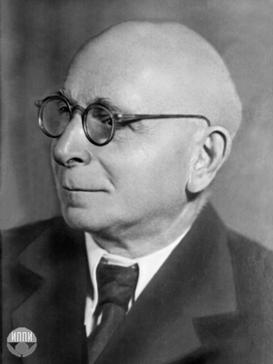
\includegraphics[width=0.3\textwidth]{bernstein.jpg}
		\end{figure}
		Sergei Natanovich Bernstein (5 marzec 1880 - 26 październik 1968)
	\end{frame}
	
	% ukrainski, a dokladniej sowiecki matematyk
	% udowodnij znane twierdzenie aprosymacyjne wereistresa (o przyblizaniu funkcji wielomianami)
	
	\begin{frame}{Wielomiany Bernsteina}
		
		\begin{definicja}
			Niech $n \in \mathbb{N}$. Definiujemy funkcje $B_i^n : [0,1] \to [0,1]$ wzorem
			\[
			B_i^n(t) = \binom{n}{i}t^i(1-t)^{n-i} \quad \text{dla każdego} \quad 0 \leqslant i \leqslant n
			\]
			Funkcja $B_i^n$ nazywana jest $i$-tym \textbf{wielomianem bazowym Bernsteina} stopnia $n$.
		\end{definicja}
		
	\end{frame}
	
	\begin{frame}{Wielomiany Bernsteina}
		\begin{uwaga}
			Dodatkowo zakładamy poniższe związki:
			
			\[
			B_i^n(0) = \binom{n}{i} 0^i (1 - 0)^{n-i} =
			\begin{cases}
				1, & i = 0, \\
				0, & 0 < i \le n,
			\end{cases}
			\]
			
			\[
			B_i^n(1) = \binom{n}{i} 1^i (1 - 1)^{n-i} =
			\begin{cases}
				0, & 0 \le i < n, \\
				1, & i = n.
			\end{cases}
			\]
			
			Wystarczy założyć, że $0^0 = 1$.
		\end{uwaga}
		
		\pause
		
		\begin{uwaga}
			Dlaczego bazowym? Ponieważ zbiór $\{{B_0^n(t),B_1^n(t), \ldots, B_n^n(t)}\}$ jest bazą przestrzeni wszystkich wielomianów stopnia conajwyżej $n$.
		\end{uwaga}  
	\end{frame}
	
	\begin{frame}{Przykład wielomianów Bernsteina}
		\begin{przyklad}
			Dla $n = 0$:
			\[
			B_0^0(t) = 1
			\]
			\pause
			Dla $n = 1$:
			\[
			B_0^1(t) = 1-t, \quad B_1^1(t) = t
			\]
			\pause
			Dla $n = 2$:
			\[
			B_0^2(t) = (1-t)^2, \quad B_1^2(t) = 2t(1-t), \quad B_2^2(t)=t^2
			\]
			\pause
			Dla $n = 3$:
			\[
			B_0^3(t)=(1-t)^3, \quad B_1^3(t)=3t(1-t)^2
			\]
			\[
			B_2^3(t)=3t^2(1-t), \quad B_3^3(t)=t^3
			\]
		\end{przyklad}
	\end{frame}
	
	\begin{frame}{Pochodna Wielomianów Bernsteina}
		Widzimy, że każdy wielomian Bernsteina jest funkcją ciągłą. Co więcej zachodzi następujące:
		\pause
		\begin{twierdzenie}
			Pochodna wielomianu Bernsteina $B_i^n$ wyraża się wzorem
			\[
			\frac{d}{dt}\Big(B_i^n(t)\Big) = n\Big(B_{i-1}^{n-1}(t) - B_i^{n-1}(t)\Big)
			\]
			co więcej każdy wielomian Bernsteina jest funkcją klasy $C^\infty$.
		\end{twierdzenie}
	\end{frame}
	
	\begin{frame}{Pochodna wielomianów Bernsteina}
		\begin{proof}
			\begin{align*}
				&\frac{d}{dt}\Bigg(\binom{n}{i}t^i(1-t)^{n-i}\Bigg) = \binom{n}{i}t^{i-1}(1-t)^{n-i} - \binom{n}{i}t^i(n-i)(1-t)^{n-i-1} \\ 
				&= n \binom{n-1}{i-1}t^{i-1}(1-t)^{n-i} - n\binom{n-1}{i}t^i (1-t)^{n-i-1} \\ &= n\Big(B_{i-1}^{n-1}(t) - B_i^{n-1}(t)\Big)
			\end{align*}
		\end{proof}
	\end{frame}
	
	\begin{frame}{Pierre Bézier}
		\begin{figure}
			\centering
			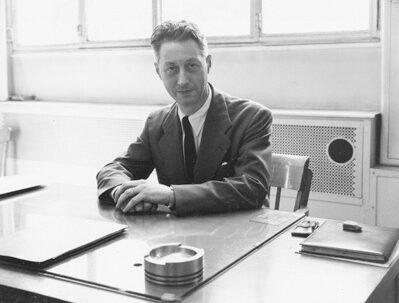
\includegraphics[width=0.55\textwidth]{pierre_bezier.jpg}
		\end{figure}
		Pierre Étienne Bézier (1 września 1910 - 25 listopad 1999)
	\end{frame}
	
	\begin{frame}{Krzywa Béziera}
		
		\begin{definicja}
			\textbf{Krzywą Béziera} stopnia $n$ w $\mathbb{R}^2$ nazywamy krzywą parametryczną $p : [0,1] \to \mathbb{R}^2$ daną wzorem
			\[
			p(t) = \sum_{i=0}^n P_i B_i^n(t)
			\]
			gdzie punkty $P_i \in \mathbb{R}^2$ nazywamy \textbf{punktami kontrolnymi} krzywej $p$.
		\end{definicja}
		
		\pause
		
		\begin{uwaga}
			Zauważmy, że zachodzą poniższe związki:
			\begin{align*}
				p(0) &= P_0 \cdot B_0^n(0) = P_0 \\
				p(1) &= P_n \cdot B_n^n(1) = P_n
			\end{align*}
		\end{uwaga}
		
	\end{frame}
	
	\begin{frame}{Krzywa Beziera II stopnia}
		\begin{przyklad}
			Krzywa Béziera drugiego stopnia:
			\[
			p(t) = P_0 \cdot (1 - t)^2 + P_1 \cdot 2 t(1 - t) + P_2 \cdot  t^2, \quad t \in [0,1]
			\]
			\begin{center}
				\begin{tikzpicture}
					% Punkty kontrolne
					\coordinate (P0) at (0,0);
					\coordinate (P1) at (1,4);
					\coordinate (P2) at (8,0);
					
					% Krzywa Béziera 2. stopnia
					\draw[blue, thick] (P0) .. controls (P1) .. (P2);
					
					% Punkty kontrolne
					\fill[red] (P0) circle (2pt) node[below left] {$P_0$};
					\fill[red] (P1) circle (2pt) node[above] {$P_1$};
					\fill[red] (P2) circle (2pt) node[below right] {$P_2$};
					
					% Linie kontrolne
					\draw[red, dashed] (P0) -- (P1);
					\draw[red, dashed] (P1) -- (P2);
				\end{tikzpicture}
			\end{center}
		\end{przyklad}
	\end{frame}
	
	\begin{frame}{Krzywa Béziera III stopnia}
		\begin{przyklad}
			Krzywa Béziera trzeciego stopnia: \[
			p(t) = P_0 \cdot (1-t)^3 + P_1 \cdot 3(1-t)^2 + P_2 \cdot 3t^2(1-t) + P_3 \cdot t^3, \quad t \in [0,1] \]
			\begin{center}
				\begin{tikzpicture}
					% Punkty kontrolne
					\coordinate (P0) at (0,0);
					\coordinate (P1) at (2,4);
					\coordinate (P2) at (6,3);
					\coordinate (P3) at (9,0);
					
					% Krzywa Béziera
					\draw[blue, thick] (P0) .. controls (P1) and (P2) .. (P3);
					
					% Punkty kontrolne
					\fill[red] (P0) circle (2pt) node[below left] {$P_0$};
					\fill[red] (P1) circle (2pt) node[above] {$P_1$};
					\fill[red] (P2) circle (2pt) node[above] {$P_2$};
					\fill[red] (P3) circle (2pt) node[below right] {$P_3$};
					
					% Linie kontrolne
					\draw[red, dashed] (P0) -- (P1);
					\draw[red, dashed] (P2) -- (P3);
					\draw[red, dashed] (P1) -- (P2);
				\end{tikzpicture}    
			\end{center}
		\end{przyklad}
	\end{frame}
	
	\begin{frame}{Własności krzywych Béziera}
		\begin{wniosek}
			Poprzez reparametryzacje dowolnego odcinka $[a,b]$ na odcinek $[0,1]$ wystarczy rozważać krzywe Béziera w ich naturalnej dziedzinie tzn. na odcinku $[0,1]$.
		\end{wniosek}
		
	\end{frame}
	
	\begin{frame}{Powłoka wypukła}
		
		\begin{definicja}
			Niech $\{P_0, P_1, \ldots P_n\}$ zbiór punktów w $\mathbb{R}^2$. Definiujemy \textbf{powłokę wypukłą} punktów $P_0, P_1, \ldots P_n$ przez
			\[
			\operatorname{conv}(P_0, P_1, \ldots, P_n) = \Bigg\{\sum_{i=0}^n \alpha_i P_i : \alpha_i \geqslant 0, \sum_{i=0}^n\alpha_i = 1\Bigg\}
			\]
			\pause
			tzn. najmniejszy wypukły zbiór, który zawiera wszystkie punkty $P_i$.
		\end{definicja}
		
	\end{frame}
	
	\begin{frame}{Powłoka wypukła}
		
		\begin{przyklad}
			\begin{center}
				\begin{tikzpicture}[scale=0.7]
					% Osie współrzędnych (zawsze widoczne)
					%	\draw[->] (0,0) -- (7,0) node[right] {$x$};
					%	\draw[->] (0,0) -- (0,7) node[above] {$y$};
					\draw[gray!20] (0,0) grid (7,7);
					% Punkty
					\only<1->{\filldraw (1,1) circle (2pt) node[below right] {$P_0=(1,1)$}};
					\only<2->{\filldraw (3,6) circle (2pt) node[above] {$P_1=(3,6)$}};
					\only<4->{\filldraw (4,3) circle (2pt) node[above right] {$P_2=(4,3)$}};
					\only<6->{\filldraw (6,2) circle (2pt) node[below right] {$P_3=(6,2)$}};
					\only<3-8>{\draw[blue, thick] (1,1) -- (3,6);}
					\only<5-7>{\draw[blue, thick] (3,6) -- (4,3);}
					\only<5-7>{\draw[blue, thick] (1,1) -- (4,3);}
					
					\only<7-8>{\draw[green, thick] (1,1) -- (6,2);}
					\only<7-8>{\draw[green, thick] (3,6) -- (6,2);}
					
					\only<8->{\draw[green, thick] (1,1) -- (3,6);}
					
				\end{tikzpicture}
			\end{center}
		\end{przyklad}
		
	\end{frame}
	
	\begin{frame}{Własności krzywych Béziera}
		
		\begin{twierdzenie}
			Niech $p(t) = \sum_{i=0}^{n}P_i B_i^n(t)$, gdzie $P_i \in \mathbb{R}^2, \, t \in  [0,1]$. Wówczas
			\[
			p(t) \in \operatorname{conv}(P_1, \ldots, P_n)
			\]
		\end{twierdzenie}
	\end{frame}
	
	\begin{frame}{Własności krzywych Béziera}
		
		\begin{przyklad}
			\begin{center}
				\begin{tikzpicture}[scale=0.7]
					
					% Siatka
					\draw[gray!20] (0,0) grid (7,7);
					
					% Punkty kontrolne
					\filldraw (1,1) circle (2pt)
					node[below right] {$P_0=(1,1)$};
					
					\filldraw (3,6) circle (2pt)
					node[above] {$P_1=(3,6)$};
					
					\filldraw (4,3) circle (2pt)
					node[above right] {$P_2=(4,3)$};
					
					\filldraw (6,2) circle (2pt)
					node[below right] {$P_3=(6,2)$};
					
					% Wielokąt kontrolny
					\draw[
					green,
					thick
					]
					(1,1) -- (3,6) -- (6,2) -- (1,1);
					
					% Krzywa Béziera stopnia 3
					\draw[
					red,
					very thick,
					domain=0:1,
					samples=150,
					smooth,
					variable=\t
					]
					plot
					(
					{
						(1-\t)*(1-\t)*(1-\t)*1
						+ 3*(1-\t)*(1-\t)*\t*3
						+ 3*(1-\t)*\t*\t*4
						+ \t*\t*\t*6
					},
					{
						(1-\t)*(1-\t)*(1-\t)*1
						+ 3*(1-\t)*(1-\t)*\t*6
						+ 3*(1-\t)*\t*\t*3
						+ \t*\t*\t*2
					}
					);
					
				\end{tikzpicture}
			\end{center}
		\end{przyklad}
		
	\end{frame}
			
%	\begin{frame}{Dowód}
%		
%		\begin{proof}
%			Mamy $p(t) = \sum_{i=0}^nP_i B_i^n(t)$. Wystarczy pokazać, że
%			\begin{itemize}
%				\item [(a)] $\alpha_i = B_i^n(t) \geqslant 0$ dla każdego $t \in [0,1]$
%				\item [(b)] $\sum_{i=0}^{n}B_i^n(t)=1$
%			\end{itemize}
%			
%			\pause 
%			
%			\begin{itemize}
%				\item [(a)] Istotnie $B_i^n(t)=\binom{n}{i}t^i(1-t)^{n-i} \geqslant 0$ dla każdego $t \in [0,1]$.
%				
%				\pause
%				
%				\item [(b)] Mamy
%				\[
%				(t+(1-t))^n=\sum_{i=0}^n\binom{n}{i}t^i(1-t)^{n-i}=\sum_{i=0}^n B_i^n(t)
%				\]
%				Zatem $\sum_{i=0}^n B_i^n(t)=1$.
%			\end{itemize}
%			
%		\end{proof} 
%	
%	\end{frame}
	
	\begin{frame}{Paul de Casteljau}
		\begin{figure}
			\centering
			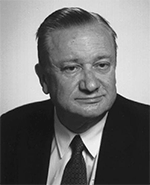
\includegraphics[width=0.3\textwidth]{casteljau.png}
		\end{figure}
		Paul de Casteljau (19 listopad 1930 – 24 marzec 2022)
	\end{frame}
	
	\begin{frame}{Algorytm de Casteljau}
		\begin{align*}
			&\text{Wejście: } P_0, \dots, P_n, \; t \in [0,1] \\
			&\text{Inicjalizacja: } P_i^0 = P_i, \quad i=0,\dots,n \\[2mm]
			&\text{Iteracja:} \\
			&\quad P_i^k = (1-t) P_i^{k-1} + t \, P_{i+1}^{k-1}, 
			\quad k=1,\dots,n, \; i=0,\dots,n-k \\[1mm]
			&\text{Wyjście: } P_0^n = B(t)
		\end{align*}
	\end{frame}
	
	\begin{frame}{Algorytm de Casteljau - krzywa II stopnia}
		\[
			P_i^0 = P_i, \qquad
			P_i^1(t) = (1-t)P_i^0 + t P_{i+1}^0, \qquad
			P_i^2(t) = (1-t)P_i^1(t) + t P_{i+1}^1(t)
		\]
		
		\begin{center}
				\begin{tikzpicture}[scale=2]
				% Punkty kontrolne
				\coordinate (P0) at (0,0);
				\coordinate (P1) at (1,1);
				\coordinate (P2) at (2,0);
				
				% Parametr
				\def\t{0.35}
				
				% Interpolacje poziomu 1
				\coordinate (Q0) at ($(P0)!\t!(P1)$);
				\coordinate (Q1) at ($(P1)!\t!(P2)$);
				
				% Interpolacja poziomu 2 (punkt krzywej)
				\coordinate (R0) at ($(Q0)!\t!(Q1)$);
				
				% Krzywa Bezier
				\onslide<4->{
					\draw[red, thick] 
					plot[domain=0:1] 
					({(1-\x)^2*0 + 2*(1-\x)*\x*1 + \x^2*2},
					{(1-\x)^2*0 + 2*(1-\x)*\x*1 + \x^2*0});
				}
				
				% Poligon kontrolny
				\onslide<1->{
					\draw[gray, thick, dashed] (P0) -- (P1) -- (P2);
					\fill (P0) circle (1pt) node[below] {$P_0$};
					\fill (P1) circle (1pt) node[above] {$P_1$};
					\fill (P2) circle (1pt) node[below] {$P_2$};
				}
				
				% Poziom 1 interpolacji
				\onslide<2->{
					\draw[blue] (Q0) -- (Q1);
					\fill[blue] (Q0) circle (1pt) node[left] {$P_0^{1}(t)$};
					\fill[blue] (Q1) circle (1pt) node[right] {$P_1^{1}(t)$};
				}
				
				% Poziom 2 interpolacji (punkt krzywej)
				\onslide<3->{
					\fill[red] (R0) circle (1.2pt) node[above] {$P_0^2(t) = B(t)$};
				}
				
			\end{tikzpicture}
		\end{center}
	\end{frame}
	
	\begin{frame}{Algorytm de Casteljau - krzywa III stopnia}
		
		\[
		\begin{aligned}
			P_i^0 &= P_i,  &P_i^1(t) &= (1-t)P_i^0 + tP_{i+1}^0,  \\
			P_i^2(t) &= (1-t)P_i^1(t) + tP_{i+1}^1(t),  &P_i^3(t) &= (1-t)P_i^2(t) + tP_{i+1}^2(t) \\
		\end{aligned}
		\]
		
		\begin{center}
			\begin{tikzpicture}[scale=1.2]
				
				% Punkty kontrolne (0. poziom)
				\coordinate (P0) at (0,0);
				\coordinate (P1) at (2,3.5);
				\coordinate (P2) at (5,3);
				\coordinate (P3) at (7,0);
				
				% Parametr
				\def\t{0.35}
				
				% Poziom 1
				\coordinate (Q0) at ($(P0)!\t!(P1)$);
				\coordinate (Q1) at ($(P1)!\t!(P2)$);
				\coordinate (Q2) at ($(P2)!\t!(P3)$);
				
				% Poziom 2
				\coordinate (R0) at ($(Q0)!\t!(Q1)$);
				\coordinate (R1) at ($(Q1)!\t!(Q2)$);
				
				% Poziom 3 (punkt krzywej)
				\coordinate (S0) at ($(R0)!\t!(R1)$);
				
				% Poligon kontrolny
				\onslide<1->{
					\draw[gray, dashed, thick] (P0) -- (P1) -- (P2) -- (P3);
					\fill (P0) circle (2pt) node[below] {$P_0$};
					\fill (P1) circle (2pt) node[above] {$P_1$};
					\fill (P2) circle (2pt) node[above] {$P_2$};
					\fill (P3) circle (2pt) node[below] {$P_3$};
				}
				
				% Poziom 1
				\onslide<2->{
					\draw[blue] (Q0) -- (Q1) -- (Q2);
					\fill[blue] (Q0) circle (2pt) node[left] {$P_0^{1}(t)$};
					\fill[blue] (Q1) circle (2pt) node[above] {$P_1^{1}(t)$};
					\fill[blue] (Q2) circle (2pt) node[right] {$P_2^{1}(t)$};
				}
				
				% Poziom 2
				\onslide<3->{
					\draw[green!70!black] (R0) -- (R1);
					\fill[green!70!black] (R0) circle (2pt) node[left] {$P_0^{2}(t)$};
					\fill[green!70!black] (R1) circle (2pt) node[right] {$P_1^{2}(t)$};
				}
				
				% Poziom 3 (punkt na krzywej)
				\onslide<4->{
					\fill[red] (S0) circle (2.2pt) node[below] {$P_0^{3}(t)=B(t)$};
				}
				
								% Krzywa Bezier 3 stopnia
				\onslide<5->{
					\draw[red, thick]
					plot[domain=0:1]
					({(1-\x)^3*0 + 3*(1-\x)^2*\x*2 + 3*(1-\x)*\x^2*5 + \x^3*7},
					{(1-\x)^3*0 + 3*(1-\x)^2*\x*3.5 + 3*(1-\x)*\x^2*3 + \x^3*0});
				}
				
			\end{tikzpicture}
		\end{center}
	\end{frame}
	
	\begin{frame}{Symulator}
		
		\begin{center}
			\qrcode[height=5cm]{https://adrianmadajewski.github.io/Oblicze2026/}
		\end{center}
		
	\end{frame}
		
	\begin{frame}{Sklejenie krzywych Béziera}
		
		\begin{problemo}
			W jaki sposób skleić ze sobą krzywe Béziera?
		\end{problemo}
		
		\pause
		
		Sklejenie krzywych (\emph{ang. spline}) może mieć różny stopień gładkości.  
		W praktyce rozróżnia się trzy poziomy gładkości:
		
		\pause
		
		\begin{itemize}
			\item $C^0$ — krzywe spotykają się w tym samym punkcie,
			\pause
			\item $C^1$ — oprócz $C^0$ zgadzają się wektory styczne,
			\pause
			\item $C^2$ — oprócz $C^1$ zgadzają się również krzywizny.
		\end{itemize}
	\end{frame}
	
	\begin{frame}{Sklejenie klasy $C^0$ krzywych Béziera}
		
		\begin{definicja}
			Niech
			\[
			p(t) = \sum_{i=0}^{n} P_i\, B_i^n(t), \qquad
			q(t) = \sum_{i=0}^{m} Q_i\, B_i^m(t), \qquad t \in [0,1], \, P_i,Q_i \in \mathbb{R}^2
			\]
			będą dwiema krzywymi Béziera stopnia $n,m$ ($n \neq m$).
			
			\pause
			
			Mówimy, że \textbf{sklejenie krzywych $p$ i $q$ jest klasy $C^0$}, jeśli zachodzi:
			\[
				p(1) = q(0).
			\]
		\end{definicja}
	\end{frame}
	
	\begin{frame}{Sklejenie klasy $C^0$ krzywych Béziera}
			
	\begin{uwaga}
		Ponieważ
		\[
		p(1) = P_n, \qquad q(0) = Q_0,
		\]
		warunek ten jest równoważny warunkowi:
		\[
		P_n = Q_0.
		\]
	\end{uwaga}
	
	\pause
	
	\begin{przyklad}
	\begin{center}
	\begin{tikzpicture}[scale=1.2]
		
		%--- First Bézier segment ---
		\coordinate (P0) at (-2,-1);
		\coordinate (P1) at (-1,0.5);
		\coordinate (P2) at (0,0); % wspólny punkt
		
		%--- Second Bézier segment (tworzy lekki spike) ---
		\coordinate (Q0) at (0,0);  % wspólny punkt
		\coordinate (Q1) at (1,0.5);
		\coordinate (Q2) at (2,-1);
		
		% First Bézier curve
		\draw[blue, thick]
		(P0) .. controls (P1) .. (P2);
		
		% Second Bézier curve
		\draw[red, thick]
		(Q0) .. controls (Q1) .. (Q2);
		
		% Control polygons (optional dashed guides)
		\draw[blue, dashed] (P0) -- (P1) -- (P2);
		\draw[red, dashed]  (Q0) -- (Q1) -- (Q2);
		
	 % Points + labels
	\fill[blue] (P0) circle (2pt) node[left] {$P_0$};
	\fill[blue] (P1) circle (2pt) node[above] {$P_1$};
	\fill[blue] (P2) circle (2pt);
	
	\fill[red] (Q1) circle (2pt) node[above] {$Q_1$};
	\fill[red] (Q2) circle (2pt) node[right] {$Q_2$};
	
	% Common point with emphasis + label
	\fill[black] (P2) circle (3pt) node[below] {$P_2 = Q_0$};
		
	\end{tikzpicture}
	\end{center}
	\end{przyklad}
	
	\end{frame}
	
	\begin{frame}{Sklejenie klasy $C^1$ krzywych Béziera}
		
		\begin{definicja}
			Niech
			\[
			p(t) = \sum_{i=0}^{n} P_i\, B_i^n(t), \qquad
			q(t) = \sum_{i=0}^{m} Q_i\, B_i^m(t), \qquad t \in [0,1], \, P_i,Q_i \in \mathbb{R}^2
			\]
			będą dwiema krzywymi Béziera stopnia $n,m$ ($n \neq m$).
			
			\pause
			Mówimy, że \textbf{sklejenie krzywych $p$ i $q$ jest klasy $C^1$},
			jeśli zachodzi:
			\[
			\text{(1)} \quad p(1) = q(0)
			\quad\text{oraz}\quad
			\text{(2)} \quad p'(1) = q'(0).
			\]
		\end{definicja}
		
		Jak wyrażą się $p'(t)$ oraz $q'(t)$?
		
	\end{frame}
	
	\begin{frame}{Pochodna Krzywej Béziera}
		\begin{twierdzenie}
			Niech
			\[
			p(t) = \sum_{i=0}^{n} P_i \, B_i^n(t), \quad t \in [0,1], \quad P_i \in \mathbb{R}^2
			\]
			będzie krzywą Béziera stopnia $n$.
			
			\pause
			
			Wówczas pochodna $p'(t)$ ma postać:
			\[
			p'(t) = n \sum_{i=0}^{n-1} (P_{i+1} - P_i)\, B_i^{n-1}(t).
			\]
		\end{twierdzenie}
	\end{frame}
	
%	\begin{frame}{Pochodna krzywej Béziera - dowód}
%		\begin{proof}
%			Z liniowości pochodnej mamy:
%			\[
%			p'(t) = \sum_{i=0}^{n} P_i \, \frac{d}{dt}\Bigg( B_i^n(t)\Bigg).
%			\]
%			
%			\pause
%			
%			Korzystamy teraz z pochodnej wielomianu Bernsteina:
%			\[
%				\frac{d}{dt}\Bigg(B_i^n(t)\Bigg) = n\left( B_{i-1}^{n-1}(t) - B_i^{n-1}(t)\right),
%			\]
%			
%			\pause
%			
%			przy czym przyjmujemy, że $B_{-1}^{n-1}(t) = B_n^{n-1}(t) = 0$ dla $t \in [0,1]$.
%			\phantom{\qedhere}
%		\end{proof}
%	\end{frame}
%	
%	\begin{frame}{Pochodna krzywej Béziera - dowód}
%		\begin{proof}
%			Podstawiając do wzoru na pochodną otrzymujemy
%			\[
%				p'(t) = \sum_{i=0}^{n} P_i \cdot n\left( B_{i-1}^{n-1}(t) - B_i^{n-1}(t)\right)
%			\]
%			
%			\pause
%			
%			Rozdzielamy na dwie sumy:
%			\[
%				p'(t) = n \sum_{i=0}^{n}P_i B_{i-1}^{n-1}(t) - n \sum_{i=0}^{n}P_i B_i^{n-1}(t).
%			\]
%			
%			\phantom{\qedhere}
%		\end{proof}
%	\end{frame}
%	
%	\begin{frame}{Pochodna krzywej Béziera - dowód}
%		\begin{proof}
%			Ponieważ $B_{-1}^{n-1}(t) = 0$ oraz $B_n^{n-1}(t) = 0$ mamy
%			\[
%			p'(t) = n \sum_{i=1}^{n}P_i B_{i-1}^{n-1}(t) - n \sum_{i=0}^{n-1}P_i B_i^{n-1}(t).
%			\]
%			
%			\pause
%			
%			Stąd re-indeksując pierwszą sumę otrzymujemy
%			\[
%				p'(t) = n \sum_{i=0}^{n-1}P_{i+1} B_{i}^{n-1}(t) - n \sum_{i=0}^{n-1}P_i B_i^{n-1}(t).
%			\]
%			
%			\pause 
%			
%			Ostatecznie
%			\[
%				p'(t) = n \sum_{i=0}^{n-1} (P_{i+1} - P_i)\, B_i^{n-1}(t).
%			\]
%
%		\end{proof}
%	\end{frame}
%
%	\begin{frame}{Druga pochodna krzywej Béziera}
%		\begin{twierdzenie}
%			Niech
%			\[
%			p(t) = \sum_{i=0}^{n} P_i \, B_i^n(t), 
%			\quad t \in [0,1], \quad P_i \in \mathbb{R}^2,
%			\]
%			będzie krzywą Béziera stopnia $n$.
%			
%			\pause
%			
%			Wówczas druga pochodna $p''(t)$ ma postać:
%			\[
%			p''(t)
%			= n(n-1) \sum_{i=0}^{n-2} 
%			\big( P_{i+2} - 2P_{i+1} + P_i \big)\, B_i^{\,n-2}(t).
%			\]
%		\end{twierdzenie}
%	\end{frame}
%	
%	\begin{frame}{Druga pochodna krzywej Béziera}
%		\begin{proof}
%			Z poprzedniego twierdzenia wiemy, że
%			\[
%			p'(t) 
%			= n \sum_{i=0}^{n-1} (P_{i+1} - P_i)\, B_i^{\,n-1}(t).
%			\]
%			
%			\pause
%			
%			Traktujemy teraz $p'(t)$ jako krzywą Béziera stopnia $n-1$:
%			\[
%			p'(t) = \sum_{i=0}^{n-1} R_i \, B_i^{\,n-1}(t),
%			\quad\text{gdzie}\quad
%			R_i := n (P_{i+1} - P_i).
%			\]
%			
%			\pause
%			
%			Zatem $R_i$ są punktami kontrolnymi krzywej $p'$.
%		\end{proof}
%	\end{frame}
%	
%	\begin{frame}{Druga pochodna krzywej Béziera}
%		\begin{proof}
%			Znowu korzystamy z faktu o pochodnej krzywej Béziera, tym razem dla $p'$:
%			\[
%			p''(t) 
%			= (n-1) \sum_{i=0}^{n-2} (R_{i+1} - R_i)\, B_i^{\,n-2}(t).
%			\]
%			
%			\pause
%			
%			Podstawiamy teraz $R_i = n (P_{i+1} - P_i)$:
%			\[
%			R_{i+1} - R_i
%			= n (P_{i+2} - P_{i+1}) - n (P_{i+1} - P_i)
%			= n \big( P_{i+2} - 2P_{i+1} + P_i \big).
%			\]
%			
%			\pause
%			
%			Zatem
%			\[
%			p''(t)
%			= n(n-1) \sum_{i=0}^{n-2} 
%			\big( P_{i+2} - 2P_{i+1} + P_i \big)\, B_i^{\,n-2}(t),
%			\]
%			co kończy dowód. \qedhere
%		\end{proof}
%	\end{frame}

	\begin{frame}{Sklejenie klasy $C^1$ krzywych Béziera}
	
	\begin{definicja}
		Niech
		\[
		p(t) = \sum_{i=0}^{n} P_i\, B_i^n(t), \qquad
		q(t) = \sum_{i=0}^{m} Q_i\, B_i^m(t), \qquad t \in [0,1], \, P_i,Q_i \in \mathbb{R}^2
		\]
		będą dwiema krzywymi Béziera stopnia $n,m$ ($n \neq m$).
		
		Mówimy, że \textbf{sklejenie krzywych $p$ i $q$ jest klasy $C^1$},
		jeśli zachodzi:
		\[
		\text{(1)} \quad p(1) = q(0)
		\quad\text{oraz}\quad
		\text{(2)} \quad p'(1) = q'(0).
		\]
		gdzie
		\[
			p'(t) = n \sum_{i=0}^{n-1} (P_{i+1} - P_i)\, B_i^{n-1}(t), \quad q'(t) = n \sum_{i=0}^{n-1} (Q_{i+1} - Q_i)\, B_i^{n-1}(t)
		\]
	\end{definicja}
	
	\end{frame}
	
	\begin{frame}{Warunek klasy $C^1$}
		
		\begin{twierdzenie}
			Przy założeniach z poprzedniej Definicji warunek (2) pociąga warunek $P_n - P_{n-1}\;\parallel\; Q_1 - Q_0$. Tzn.
			\[
				p'(1) = q'(0) \implies P_n - P_{n-1} \;\parallel\; Q_1 - Q_0
			\]
		\end{twierdzenie}
		
		\pause
		
		\begin{uwaga}
			Równość $P_n - P_{n-1} = Q_1 - Q_0$ zachodzi jeśli krzywe $p,q$ mają ten sam stopień. Tzn. jeśli $n = m$.
		\end{uwaga}
		
		\pause
		
		\begin{uwaga}
			Podobną własność można wykazać dla sklejenia funkcji wyższej klasy np. $C^2, C^3, \ldots$.
		\end{uwaga}
	\end{frame}
	
\begin{frame}{Warunek klasy $C^1$}
	
	\begin{proof}
		
		Ze wzoru na pochodną krzywej Béziera mamy
		\[
		p'(t)
		= n \sum_{i=0}^{n-1} (P_{i+1}-P_i)\, B_i^{\,n-1}(t).
		\]
		
		\pause
		W punkcie $t=1$ jedynym niezerowym wielomianem Bernsteina stopnia $n-1$ jest
		\[
		B_{n-1}^{\,n-1}(1) = 1.
		\]
		
		\pause
		Zatem
		\[
		p'(1) = n(P_n - P_{n-1}).
		\]
		
		\pause
		Analogicznie,
		\[
		q'(0) = m(Q_1 - Q_0).
		\]
		\renewcommand{\qedsymbol}{} % temporary disable
	\end{proof}
	
\end{frame}

% --------------------------------------------------------------
% FRAME 2 — krok 2
% --------------------------------------------------------------
\begin{frame}{Warunek klasy $C^1$}
	
	\begin{proof}
		
		Warunek $p'(1)=q'(0)$ daje:
		\[
		n(P_n - P_{n-1})
		= m(Q_1 - Q_0).
		\]
		
		\pause
		Ponieważ $n > 0$, możemy podzielić obie strony przez $n$:
		\[
		P_n - P_{n-1}
		= \frac{m}{n}\,(Q_1 - Q_0).
		\]
		
		\pause
		Są to więc dwa wektory różniące się jedynie \emph{niezerowym skalarem}. 
		
		\pause 
		
		Zatem:
		\[
			P_n - P_{n-1} \parallel Q_1 - Q_0.
		\]
	\end{proof}
	
\end{frame}

\begin{frame}{Przykład ciągłości klasy $C^1$}
	\begin{przyklad}
		\begin{center}
			\begin{tikzpicture}[scale=1.3]
				
				% --- First Bézier segment ---
				\coordinate (P0) at (-3,-1);
				\coordinate (P1) at (-1,1.2);
				\coordinate (P2) at (0,0);  % wspólny punkt
				
				% Kierunek stycznej (wektor)
				\coordinate (TdirA) at (0.9,-1.08);  % krótszy wektor
				\coordinate (TdirB) at (1.4,-1.68);  % dłuższy wektor
				
				% --- Second Bézier segment ---
				\coordinate (Q0) at (0,0);   
				\coordinate (Q1) at ($(Q0)+(0.8,-0.96)$);
				\coordinate (Q2) at (2.7,-1);
				
				% --- Bézier curves ---
				\draw[blue, thick] (P0) .. controls (P1) .. (P2);
				\draw[red,  thick] (Q0) .. controls (Q1) .. (Q2);
				
				% --- Control polygons ---
				\draw[blue, dashed] (P0) -- (P1) -- (P2);
				\draw[red,  dashed] (Q0) -- (Q1) -- (Q2);
				
				% --- Points ---
				\fill[blue]  (P0) circle (2pt) node[left] {$P_0$};
				\fill[blue]  (P1) circle (2pt) node[above] {$P_1$};
				
				\fill[black] (P2) circle (3pt) node[below right] {$P_2 = Q_0$};
				
				\fill[red]   (Q1) circle (2pt) node[right] {$Q_1$};
				\fill[red]   (Q2) circle (2pt) node[right] {$Q_2$};
				
				% --- Tangent vectors ---
				% Both tangent vectors are collinear (same line), but labels are shifted
				\draw[very thick, blue!70, ->] (P2) -- ($(P2)+(TdirA)$);
				\draw[very thick, red!70,  ->,dashed] (P2) -- ($(P2)+(TdirB)$);
				
				% Labels shifted perpendicular for readability
				\node[blue!70] at ($(P2)+(TdirA)+(0.25,0.35)$) {$p'(1)$};
				\node[red!70]  at ($(P2)+(TdirB)+(-0.35,-0.35)$) {$q'(0)$};
				
			\end{tikzpicture}
		\end{center}
	\end{przyklad}
\end{frame}

%\begin{frame}{Ciągłość klasy $C^2$ dla krzywych Béziera}
%	
%	\begin{definicja}
%		Niech
%		\[
%		p(t) = \sum_{i=0}^{n} P_i\, B_i^n(t), \qquad
%		q(t) = \sum_{i=0}^{m} Q_i\, B_i^m(t), \qquad t \in [0,1], \, P_i,Q_i \in \mathbb{R}^2
%		\]
%		będą dwiema krzywymi Béziera stopnia $n,m$ ($n \neq m$).
%		
%		\pause
%		Mówimy, że \textbf{sklejnie krzywych $p$ i $q$ jest klasy $C^2$},  
%		jeśli spełnione są warunki:
%		\[
%			p(1)=q(0),
%			\qquad
%			p'(1)=q'(0),
%			\qquad
%			p''(1)=q''(0).
%		\]
%		\end{definicja}
%	
%\end{frame}
%
%\begin{frame}{Warunek klasy $C^2$}
%	\begin{twierdzenie}
%			Przy założeniach poprzedniej Definicji zachodzi następująca implikacja:
%			\[
%				p''(1) = q''(0) \implies P_n - 2P_{n-1} + P_{n - 2} \parallel Q_2 - 2Q_1 + Q_0
%			\]
%	\end{twierdzenie}	
%	
%	\pause 
%	
%	\begin{uwaga}
%		Równość oczywiście zachodzi, jeśli stopnie krzywych Béziera są równe. Tzn $n = m$. 
%	\end{uwaga}
%\end{frame}

\begin{frame}{Ciągłość geometryczna $G^k$}
	\begin{wniosek}
		Powyższe warunek odzwierciedlą ciągłość w klasycznym sensie, ale do samej \textit{wizualizacji} krzywej nie potrzebujemy tak wiele. Wprowadza się więc pojęcie \textbf{ciągłości geometrycznej} oznaczanej przez $G^k$.
	\end{wniosek}
	
	\pause
	
	\begin{definicja}
		Powiemy, że dwie krzywe są klasy $G^k$ jeśli spełniony jest warunek:
		\[
			p^{(j)}(1) \parallel q^{(j)}(0),
			\qquad j = 0,1,\dots,k.
		\]
		
		\pause
		Ciągłość geometryczna $G^k$ jest zatem słabsza niż ciągłość klasyczna $C^k$,
		ponieważ nie wymaga równości pochodnych, a jedynie zgodności ich kierunku.
	\end{definicja}
\end{frame}

\begin{frame}
	Teraz będzie już mniej formalnie. 
	
	\pause
	
	\begin{definicja}
		Przez \texttt{glyph} rozumiemy najmniejszą jednostkę graficzną w foncie - kontur (lub zestaw konturów), bitmapa lub inna forma rysunku, który odpowiada znakowi lub elementowi znaku. 
	\end{definicja}
	
		\begin{center}
			\begin{tikzpicture}
				\node {\fontsize{180}{180}\selectfont Ä};
			\end{tikzpicture}
		\end{center}
\end{frame}

\begin{frame}{Jak fonty przechowują krzywe?}
	
	Każda litera (każdy \texttt{glyph}) w czcionce jest zapisana m.in. jako:
	
	\pause
	\begin{itemize}
		\item \textbf{kontur} (zbiór zamkniętych krzywych), 
		\pause \item \textbf{punkty on-curve} -- leżą dokładnie na konturze, 
		\pause \item \textbf{punkty off-curve} -- punkty kontrolne krzywych Béziera. 
	\end{itemize}
	
	\pause
	Font \textbf{nie przechowuje żadnych wzorów} ani równań.  
	Zapisane są wyłącznie:
	\begin{itemize}
		\item współrzędne punktów,
		\item flagi (on/off curve),
		\item instrukcje, jak te punkty połączyć.
	\end{itemize}
	
	\pause
	Dopiero rasteryzator (np. FreeType) odtwarza krzywe Béziera i rysuje literę.
\end{frame}

%\begin{frame}{Struktura glifu w czcionce (tabela \texttt{glyf})}
%	
%	\begin{itemize}
%		\item liczba konturów,
%		\item bounding box: $x_{\min}, y_{\min}, x_{\max}, y_{\max}$,
%		\item tablice współrzędnych punktów,
%		\item tablica flag: on-curve / off-curve,
%		\item ewentualne podpowiedzi dla rasteryzatora.
%	\end{itemize}
%	
%	\pause
%	Dla glifów złożonych tabela \texttt{glyph} zawiera odwołania  
%	do innych glifów + ich transformacje (skalowanie, przesunięcie, obrót).
%\end{frame}

\begin{frame}{Różne formaty czcionek}
	
	\textbf{TrueType (Apple)} \texttt{.ttf} (TrueType outlines)  
	\begin{itemize}
		\item używa \textbf{krzywych Béziera drugiego stopnia},
	\end{itemize}
	
	\pause
	\textbf{PostScript (Adobe)} \texttt{.cff} (PostScript outlines)
	\begin{itemize}
		\item używa \textbf{krzywych Béziera trzeciego stopnia},
	\end{itemize}
	
	\pause
	\textbf{OpenType}  
	\begin{itemize}
		\item format kontenerowy,
		\item może zawierać glyph w wersji \texttt{.ttf} 
		lub \texttt{.cff}.
	\end{itemize}
\end{frame}

\begin{frame}{Przykłady liczby glifów w fontach}
	
	\begin{itemize}
		\item Debrosee Font — ok. 300 glifów,
		\item Times New Roman — ok. 4000 glifów,
		\item nowoczesne fonty Unicode — często 3000–5000 glifów,
		\item fonty CJK — nawet 20 000 glifów.
	\end{itemize}
	
	\begin{figure}[h]
		\centering
		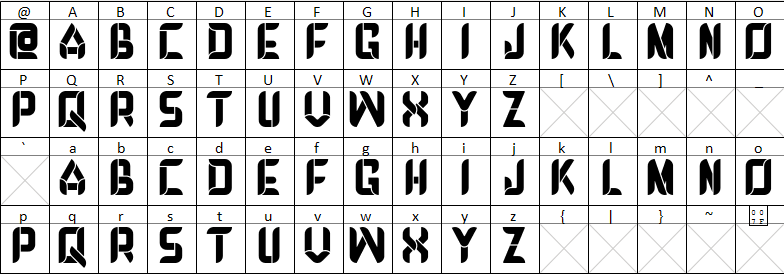
\includegraphics[width=0.5\textwidth]{debrosee.png}
	\end{figure}
	
		\begin{figure}[h]
		\centering
		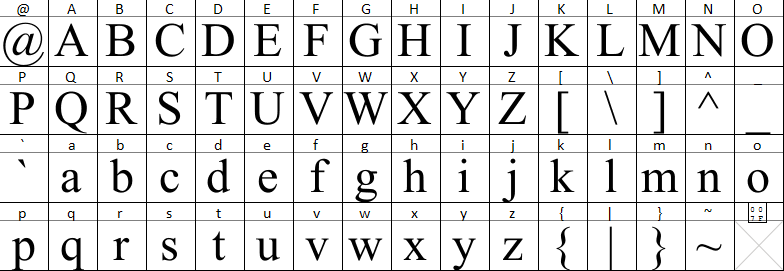
\includegraphics[width=0.5\textwidth]{times_new_roman.png}
	\end{figure}
	
\end{frame}

\begin{frame}{Przykład pojedynczego glifu w edytorze FontForge}
	
	\begin{center}
		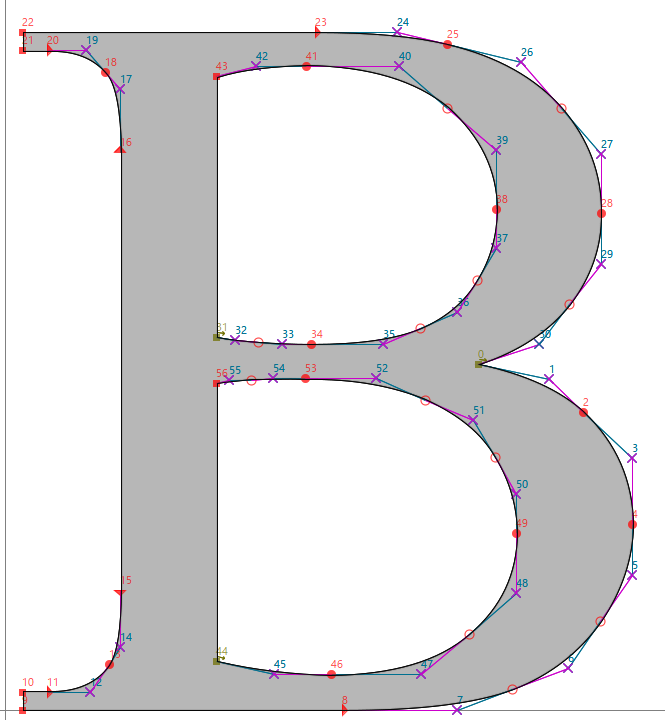
\includegraphics[width=0.5\textwidth]{glyph_B_fontforge.png}
	\end{center}
		
\end{frame}

\begin{frame}{Przykład pojedynczego glifu w Python}
	\begin{figure}
		\centering
		\begin{minipage}{0.40\textwidth}
			\centering
			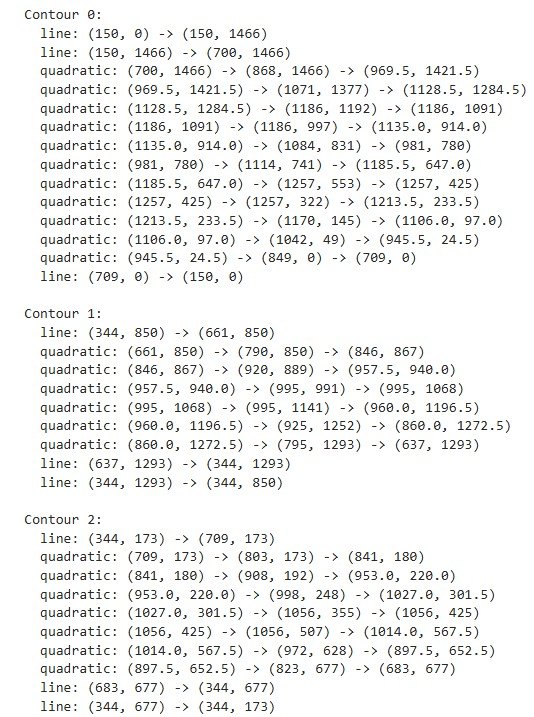
\includegraphics[width=\linewidth]{python_bezier}
			\caption{Stuktura glifu}
		\end{minipage}
		\hfill
		\begin{minipage}{0.45\textwidth}
			\centering
			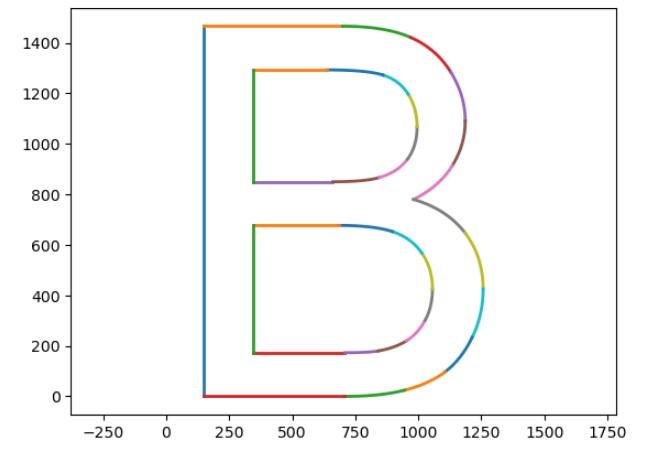
\includegraphics[width=\linewidth]{python_wykres}
			\caption{Wynik narysowania krzywych}
		\end{minipage}
	\end{figure}
\end{frame}

\begin{frame}{Rasteryzacja}
		\begin{center}
		
\includegraphics[width=0.5\textwidth]{wiadro.png}
	\end{center}
\end{frame}

%\begin{frame}{Rasteryzacji}
%	
%	Niech
%	\[
%	\Gamma = \{\gamma_1, \dots, \gamma_k\}
%	\]
%	będzie zbiorem zamkniętych konturów w $\mathbb{R}^2$.
%	
%	\pause
%	
%	Dla punktu $P \in \mathbb{R}^2$ rozważamy półprostą
%	\[
%	R = \{P + t(1,0) : t \ge 0\}.
%	\]
%	
%	\pause
%	
%	Definiujemy liczbę owinięć:
%	\[
%	W(P) = \sum_{i=1}^k W_i(P),
%	\]
%	gdzie $W_i(P)$ zlicza przecięcia $\gamma_i$ z $R$ z wagą
%	$+1$ dla przejścia w górę i $-1$ dla przejścia w dół.
%	
%	\pause
%	
%	\textbf{Kryterium non-zero winding rule}
%	\[
%	W(P) \neq 0 \Rightarrow P \text{ wewnątrz}, 
%	\qquad
%	W(P) = 0 \Rightarrow P \text{ na zewnątrz}.
%	\]
%	
%\end{frame}

\begin{frame}{Non-zero winding rule w praktyce}
	Niech $P$ będzie punktem w obrębie konturu krzywej. 
	
	\pause 
	
\begin{center}
	\begin{tikzpicture}[scale=1.2, thick]
		
		% --- 1. Najpierw rysujemy kontury ---
		\onslide<1->{
			% Kontur zewnętrzny (CCW)
			\draw[blue, line width=1.4pt] (0,0) circle (2);
			\node[blue] at (0,2.4) {\small kontur zewnętrzny};
			
			% Strzałka kierunku CCW
			\draw[blue, ->] (0+2,0) arc (0:30:2);
			
			% Kontur wewnętrzny (CW)
			\draw[red, line width=1.4pt] (0,0) circle (1);
			\node[red] at (0,-1.4) {\small kontur wewnętrzny};
			
			% Strzałka kierunku CW
			\draw[red, <-] (0+1,0) arc (0:40:1);
		}
		
		% --- 2. Potem punkt P ---
		\onslide<2->{
			\coordinate (P) at (-3,0);
			\fill (P) circle (2.5pt);
			\node[below] at (P) {$P$};
		}
		
		% --- 3. Potem półprosta ---
		\onslide<3->{
			\draw[gray!60, very thick, ->] (P) -- (4,0) node[right] {$R$};
		}
		
		% --- 4. Na końcu przecięcia i wartości +1, -1 ---
		\onslide<4->{
			% Zewnętrzny +1
			\fill[blue] ( -3+1, 0 ) circle (2pt);
			\node[above] at (-2,0.1) {$+1$};
			
			% Zewnętrzny +1
			\fill[blue] ( 2, 0 ) circle (2pt);
			\node[above] at (2,0.1) {$+1$};
			
			% Wewnętrzny -1
			\fill[red] ( -3+2, 0 ) circle (2pt);
			\node[below] at (-1,-0.1) {$-1$};
			
				% Wewnętrzny -1
			\fill[red] ( 1, 0 ) circle (2pt);
			\node[below] at (1,-0.1) {$-1$};
		}
		
	\end{tikzpicture}
\end{center}

\onslide<5->{
	$W(P) = 0$, zatem punkt $P$ jest punktem zewnętrznym. 
}

\end{frame}

\begin{frame}{Non-zero winding rule w praktyce}
\begin{center}
	\begin{tikzpicture}[scale=1.2, thick]
		
		% --- 1. Najpierw rysujemy kontury ---
		\onslide<1->{
			% Kontur zewnętrzny (CCW)
			\draw[blue, line width=1.4pt] (0,0) circle (2);
			\node[blue] at (0,2.4) {\small kontur zewnętrzny};
			
			% Strzałka kierunku CCW
			\draw[blue, ->] (0+2,0) arc (0:30:2);
			
			% Kontur wewnętrzny (CW)
			\draw[red, line width=1.4pt] (0,0) circle (1);
			\node[red] at (0,-1.4) {\small kontur wewnętrzny};
			
			% Strzałka kierunku CW
			\draw[red, <-] (0+1,0) arc (0:40:1);
		}
		
		% --- 2. Potem punkt P ---
		\onslide<2->{
			\coordinate (P) at (-1.5,0);
			\fill (P) circle (2.5pt);
			\node[below] at (P) {$P$};
		}
		
		% --- 3. Potem półprosta ---
		\onslide<3->{
			\draw[gray!60, very thick, ->] (P) -- (4,0) node[right] {$R$};
		}
		
		% --- 4. Na końcu przecięcia i wartości +1, -1 ---
		\onslide<4->{			
			% Zewnętrzny +1
			\fill[blue] ( 2, 0 ) circle (2pt);
			\node[above] at (2,0.1) {$+1$};
			
			% Wewnętrzny -1
			\fill[red] ( -3+2, 0 ) circle (2pt);
			\node[below] at (-1,-0.1) {$-1$};
			
			% Wewnętrzny -1
			\fill[red] ( 1, 0 ) circle (2pt);
			\node[below] at (1,-0.1) {$-1$};
		}
		
	\end{tikzpicture}
\end{center}

\onslide<5->{
	$W(P) = -1$, zatem punkt $P$ jest punktem wewnętrznym. 
}
\end{frame}

\begin{frame}{Funkcja charakterystyczna glifu}
	
	\begin{definicja}
		Za pomocą non-zero winding rule definiujemy funkcję
		\[
		\chi_G : \mathbb{R}^2 \to \{0,1\}
		\]
		daną przez:
		\[
		\chi_G(P) =
		\begin{cases}
			1, & \text{jeśli } P \text{ leży wewnątrz glifu}, \\
			0, & \text{w przeciwnym razie}.
		\end{cases}
		\]
	\end{definicja}
	
	\pause
	
	\begin{wniosek}
		Funkcja $\chi_G$ jest jedyną informacją geometryczną potrzebną
		do rasteryzacji glifu.
	\end{wniosek}

\end{frame}

%\begin{frame}{Coverage}
%	
%	Dla piksela $(x,y)$ rozważamy jego obszar
%	\[
%	A_{x,y} = [x, x+1] \times [y, y+1].
%	\]
%	
%	\pause
%	
%	Wybieramy $N$ punktów próbkowania $\{(x_k,y_k)\}_{k=1}^N \subset A_{x,y}$.
%	
%	\pause
%	
%	\begin{definicja}
%			Coverage piksela to średnia wartości funkcji charakterystycznej glifu:
%		\[
%		\operatorname{coverage}(x,y)
%		=
%		\frac{1}{N}
%		\sum_{k=1}^{N}
%		\chi_G(x_k,y_k).
%		\]
%		
%	\end{definicja}
%\end{frame}

%\begin{frame}{Antyaliasing}
%	
%		\begin{figure}[h]
%		\centering
%		\includegraphics[width=0.3\textwidth]{antialiasing.png}
%	\end{figure}
%	
%
%\end{frame}

%\begin{frame}{Antyaliasing - matematyczniej}
%	Dla piksela $(x,y)$ rozważamy obszar
%	\[
%	A_{x,y} = [x,x+1]\times [y,y+1],
%	\]
%	oraz próbki $\{(x_k, y_k)\}_{k=1}^N \subset A_{x,y}$.
%	
%	\pause
%	
%	Definiujemy współczynnik wypełnienia:
%	\[
%	\alpha_{x,y}
%	=
%	\frac{1}{N}\sum_{k=1}^N \chi_G(x_k, y_k).
%	\]
%	
%	\pause
%	
%	\textbf{Wartość Antyaliasingu} to właśnie wartość $\alpha_{x,y}$.
%	
%	\pause
%	
%	Jeżeli krawędź glifu przechodzi przez piksel,
%	część próbek leży wewnątrz, a część na zewnątrz,
%	co daje wartość pośrednią $0 < \alpha_{x,y} < 1$.
%\end{frame}
%
%\begin{frame}{Rezultat}
%	\centering
%	{\usefont{T1}{lmss}{b}{n}\scalebox{10}{B}}
%\end{frame}

\begin{frame}{Antyaliasing}
	
	\begin{center}
		\begin{tikzpicture}[scale=0.5]
			
			% =========================
			% LEWA: ALIASING (zawsze widoczny)
			% =========================
			\begin{scope}[xshift=-5cm]
				
				\foreach \x/\y in {
					0/0, 1/0, -1/0, 0/1, 0/-1,
					1/1, 1/-1, -1/1, -1/-1,
					2/0, -2/0, 0/2, 0/-2
				}{
					\fill[black] (\x,\y) rectangle ++(1,1);
				}
				
				\draw[step=1cm,gray!30] (-3,-3) grid (4,4);
				\node at (0,-4) {Aliasing};
				
			\end{scope}
			
			% =========================
			% PRAWA: ANTYALIASING (dopiero od slajdu 2)
			% =========================
			\onslide<2->{
				\begin{scope}[xshift=5cm]
					
					\foreach \x/\y in {
						0/0, 1/0, -1/0, 0/1, 0/-1
					}{
						\fill[black] (\x,\y) rectangle ++(1,1);
					}
					
					\foreach \x/\y in {
						1/1, 1/-1, -1/1, -1/-1
					}{
						\fill[black!60] (\x,\y) rectangle ++(1,1);
					}
					
					\foreach \x/\y in {
						2/0, -2/0, 0/2, 0/-2
					}{
						\fill[black!30] (\x,\y) rectangle ++(1,1);
					}
					
					\draw[step=1cm,gray!30] (-3,-3) grid (4,4);
					\node at (0,-4) {Antyaliasing};
					
				\end{scope}
			}
			
		\end{tikzpicture}
	\end{center}
	
	\only<3>{
	\textbf{Antyaliasing} w rasteryzacji czcionek
	to operacja próbkowania co dzieję się w otoczeniu konkretnego piksela. 
	}
	
\end{frame}

\begin{frame}{Rezultat}
	\centering
	{\usefont{T1}{lmss}{b}{n}\scalebox{10}{B}}
\end{frame}

\begin{frame}{Materiały}
	
	\begin{center}
		Materiały dostępne są w repozytorium:
	\end{center}
	
	\vspace{0.4cm}
	
	\begin{center}
		\texttt{\small https://github.com/AdrianMadajewski/Oblicze2026}
	\end{center}
	
	\vspace{0.8cm}
	
	\begin{center}
		\qrcode[height=3.5cm]{https://github.com/AdrianMadajewski/Oblicze2026}
	\end{center}
	
\end{frame}

\begin{frame}[allowframebreaks]{Bibliografia}
	\small
	\begin{thebibliography}{9}		
		\bibitem{farin}
		G.~Farin.
		\newblock {\em Curves and Surfaces for Computer-Aided Geometric Design}.
		\newblock Academic Press, 2002.
		
		\bibitem{prautzsch}
		H.~Prautzsch, W.~Boehm, and M.~Paluszny.
		\newblock {\em B{\'e}zier and B-Spline Techniques}.
		\newblock Springer, 2002.
		
		%\bibitem{foley}
		%J.~D. Foley, A.~van Dam, S.~K. Feiner, and J.~F. Hughes.
		%\newblock {\em Computer Graphics: Principles and Practice}.
		%\newblock Addison-Wesley, 3rd edition, 2013.
		
		\bibitem{truetype}
		Apple Inc.
		\newblock {\em TrueType Reference Manual}, 1990.
		\newblock Dostępne online.
		
		\bibitem{freetype}
		The FreeType Project.
		\newblock {\em FreeType 2 Documentation}, 2024.
		\newblock Dostępne online.
		
	%	\bibitem{Ljubljana}
	%	A.~Madajewski.
	%	\newblock {\em Notatki własne z wykładów w ramach Mathematics in Ljubljana 2025}.
		
		%\bibitem{li_liu}
		%J.~Li and C.~Liu.
		%\newblock {\em Smoothing Connected Bézier Curves and Surfaces through Optimal Adjustment of the Control Points}.
		%\newblock Journal of Information \& Computational Science, 2013.
		
	\end{thebibliography}
\end{frame}

\end{document}